\documentclass[crop,tikz]{standalone}

\usepackage{tikz}
\usetikzlibrary{calc, backgrounds, decorations.pathreplacing}


\definecolor{pastelblue}{RGB}{81,96,145}
\definecolor{pastellblue}{RGB}{116,190,193}
\definecolor{pastellgreen}{RGB}{173,235,190}
\definecolor{pastellyellow}{RGB}{238,243,173}
\definecolor{pastellorange}{RGB}{243,213,173}

\begin{document}

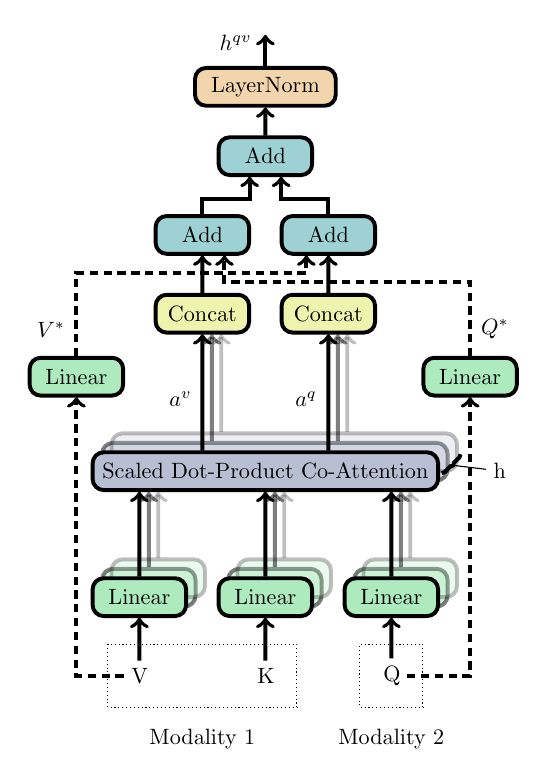
\begin{tikzpicture}[scale=.8, every node/.style={scale=.8}]
\tikzstyle{sqr} = [rectangle, rounded corners, minimum width=1cm, text width=1.25cm, minimum height=.6cm,text centered, draw=black, line width=.5mm]
\tikzstyle{rect} = [rectangle, rounded corners, minimum width=1cm, minimum height=2cm,text centered, draw=black, line width=.5mm]

\node (l1) [sqr, fill=pastellgreen] {Linear};
\begin{scope}[on  background layer]
\node (l11) [sqr, fill=pastellgreen, xshift=.15cm, yshift=.15cm, opacity=.5] {};
\node (l12) [sqr, fill=pastellgreen, xshift=.3cm, yshift=.3cm, opacity=.25] {};
\end{scope}

\node (l2) [sqr, fill=pastellgreen, right of=l1, xshift=1cm] {Linear};
\begin{scope}[on  background layer]
\node (l21) [sqr, fill=pastellgreen, right of=l1, xshift=1.15cm, yshift=.15cm, opacity=.5] {};
\node (l22) [sqr, fill=pastellgreen, right of=l1, xshift=1.3cm, yshift=.3cm, opacity=.25] {};
\end{scope}

\node (l3) [sqr, fill=pastellgreen, right of=l2, xshift=1cm] {Linear};
\begin{scope}[on  background layer]
\node (l31) [sqr, fill=pastellgreen, right of=l2, xshift=1.15cm, yshift=.15cm, opacity=.5] {};
\node (l32) [sqr, fill=pastellgreen, right of=l2, xshift=1.3cm, yshift=.3cm, opacity=.25] {};
\end{scope}

\node (coattn) [sqr, fill=pastelblue!40, above of=l2, xshift=0cm, text width=5.25cm, yshift=1cm] {Scaled Dot-Product Co-Attention};
\begin{scope}[on  background layer]
\node (coattn1) [sqr, fill=pastelblue!40, above of=l2, xshift=.15cm, text width=5.25cm, yshift=1.15cm, opacity=.5] {};
\node (coattn2) [sqr, fill=pastelblue!40, above of=l2, xshift=.3cm, text width=5.25cm, yshift=1.3cm, opacity=.25] {};
\end{scope}

\node (add1) [sqr, fill=pastellyellow, above of=coattn, yshift=1.5cm, xshift=-1cm] {Concat};
\node (add2) [sqr, fill=pastellyellow, above of=coattn, yshift=1.5cm, xshift=1cm] {Concat};

\node (add4) [sqr, fill=pastellblue!70, above of=add1, yshift=.25cm] {Add};
\node (add5) [sqr, fill=pastellblue!70, above of=add2, yshift=.25cm] {Add};

\node (add3) [sqr, fill=pastellblue!70, above of=add4, yshift=.25cm, xshift=1cm] {Add};

\node (norm) [sqr, fill=pastellorange, above of=add3, yshift=.1cm, text width=2cm] {LayerNorm};

\node (l4) [sqr, fill=pastellgreen, above of=coattn, xshift=-3cm, yshift=.5cm] {Linear};
\node (l5) [sqr, fill=pastellgreen, above of=coattn, xshift=3.25cm, yshift=.5cm] {Linear};

\node (Q) [text width=.25cm, below of=l3, yshift=-.25cm] {Q};
\node (K) [text width=.25cm, below of=l2, yshift=-.25cm] {K};
\node (V) [text width=.25cm, below of=l1, yshift=-.25cm] {V};
\node (Vstar) [text width=.25cm, above of=l4, yshift=-.25cm, xshift=-.5cm] {$V^*$};
\node (Qstar) [text width=.25cm, above of=l5, yshift=-.25cm, xshift=.3cm] {$Q^*$};


\draw[->, line width=.5mm] (l1) -- ($(coattn.south) + (-2cm, 0)$);
\draw[->, line width=.5mm, opacity=.5] (l11) -- ($(coattn.south) + (-1.85cm, 0)$);
\draw[->, line width=.5mm, opacity=.25] (l12) -- ($(coattn.south) + (-1.7cm, 0)$);

\draw[->, line width=.5mm] (l2) -- ($(coattn.south) + (0, 0)$);
\draw[->, line width=.5mm, opacity=.5] (l21) -- ($(coattn.south) + (.15cm, 0)$);
\draw[->, line width=.5mm, opacity=.25] (l22) -- ($(coattn.south) + (.3cm, 0)$);

\draw[->, line width=.5mm] (l3) -- ($(coattn.south) + (2cm, 0)$);
\draw[->, line width=.5mm, opacity=.5] (l31) -- ($(coattn.south) + (2.15cm, 0)$);
\draw[->, line width=.5mm, opacity=.25] (l32) -- ($(coattn.south) + (2.3cm, 0)$);

\draw[->, line width=.5mm] ($(coattn.north) + (-1, 0)$) -- ($(add1.south) + (0, 0)$);
\draw[->, line width=.5mm, opacity=.5] ($(coattn1.north) + (-1, 0)$) -- ($(add1.south) + (.15cm, 0)$);
\draw[->, line width=.5mm, opacity=.25] ($(coattn2.north) + (-1, 0)$) -- ($(add1.south) + (.3cm, 0)$);

\draw[->, line width=.5mm] ($(coattn.north) + (1, 0)$) -- ($(add2.south) + (0, 0)$);
\draw[->, line width=.5mm, opacity=.5] ($(coattn1.north) + (1, 0)$) -- ($(add2.south) + (.15cm, 0)$);
\draw[->, line width=.5mm, opacity=.25] ($(coattn2.north) + (1, 0)$) -- ($(add2.south) + (.3cm, 0)$);

\draw[->, line width=.5mm] (add1) -- (add4);
\draw[->, line width=.5mm] (add2) -- (add5);
\draw[->, line width=.5mm] (add4.north) |- +(.25, .25) -| ($(add3.south) + (-.25, 0)$);
\draw[->, line width=.5mm] (add5.north) |- +(-.25, .25) -| ($(add3.south) + (.25, 0)$);

\draw[->, line width=.5mm, densely dashed] (l4) |- +(1, 1.65) -| ($(add5.south) + (-.35, 0)$);
\draw[->, line width=.5mm, densely dashed] (l5) |- +(-1, 1.5) -| ($(add4.south) + (.35, 0)$);

\draw[->, line width=.5mm] (V) -- (l1);
\draw[->, line width=.5mm] (K) -- (l2);
\draw[->, line width=.5mm] (Q) -- (l3);

\draw[->, line width=.5mm, densely dashed] (V) -| (l4);
\draw[->, line width=.5mm, densely dashed] (Q) -| (l5);

\draw[->, line width=.5mm] (norm.north) -- +(0, .5);
\draw[->, line width=.5mm] (add3) -- (norm);

\draw [decorate,decoration={brace,amplitude=1pt,mirror,raise=1pt},yshift=0pt, line width=.5mm] (coattn.east) -- (coattn2.east);
\node (h) [text width=.25cm, right of=coattn, yshift=0, xshift=2.75cm] {h};
\draw [-] ($(coattn.east) + (.15cm, .1cm)$) -- (h);

\node (av) [text width=.25cm, above of=coattn, yshift=.15cm, xshift=-1.4cm] {$a^v$};
\node (aq) [text width=.25cm, above of=coattn, yshift=.15cm, xshift=.6cm] {$a^q$};
\node (out) [text width=.25cm, above of=norm, yshift=-.3cm, xshift=-.6cm] {$h^{qv}$};

\draw[densely dotted] (2.5, -1.75) rectangle node[yshift=-1cm] {Modality $1$} (-.5, -.75);
\draw[densely dotted] (4.5, -1.75) rectangle node[yshift=-1cm] {Modality $2$} (3.5, -.75);

\end{tikzpicture}

\end{document}